\documentclass[tikz,border=10pt]{standalone}
\usepackage{amsmath}
\usetikzlibrary{arrows.meta, positioning, calc}

\begin{document}
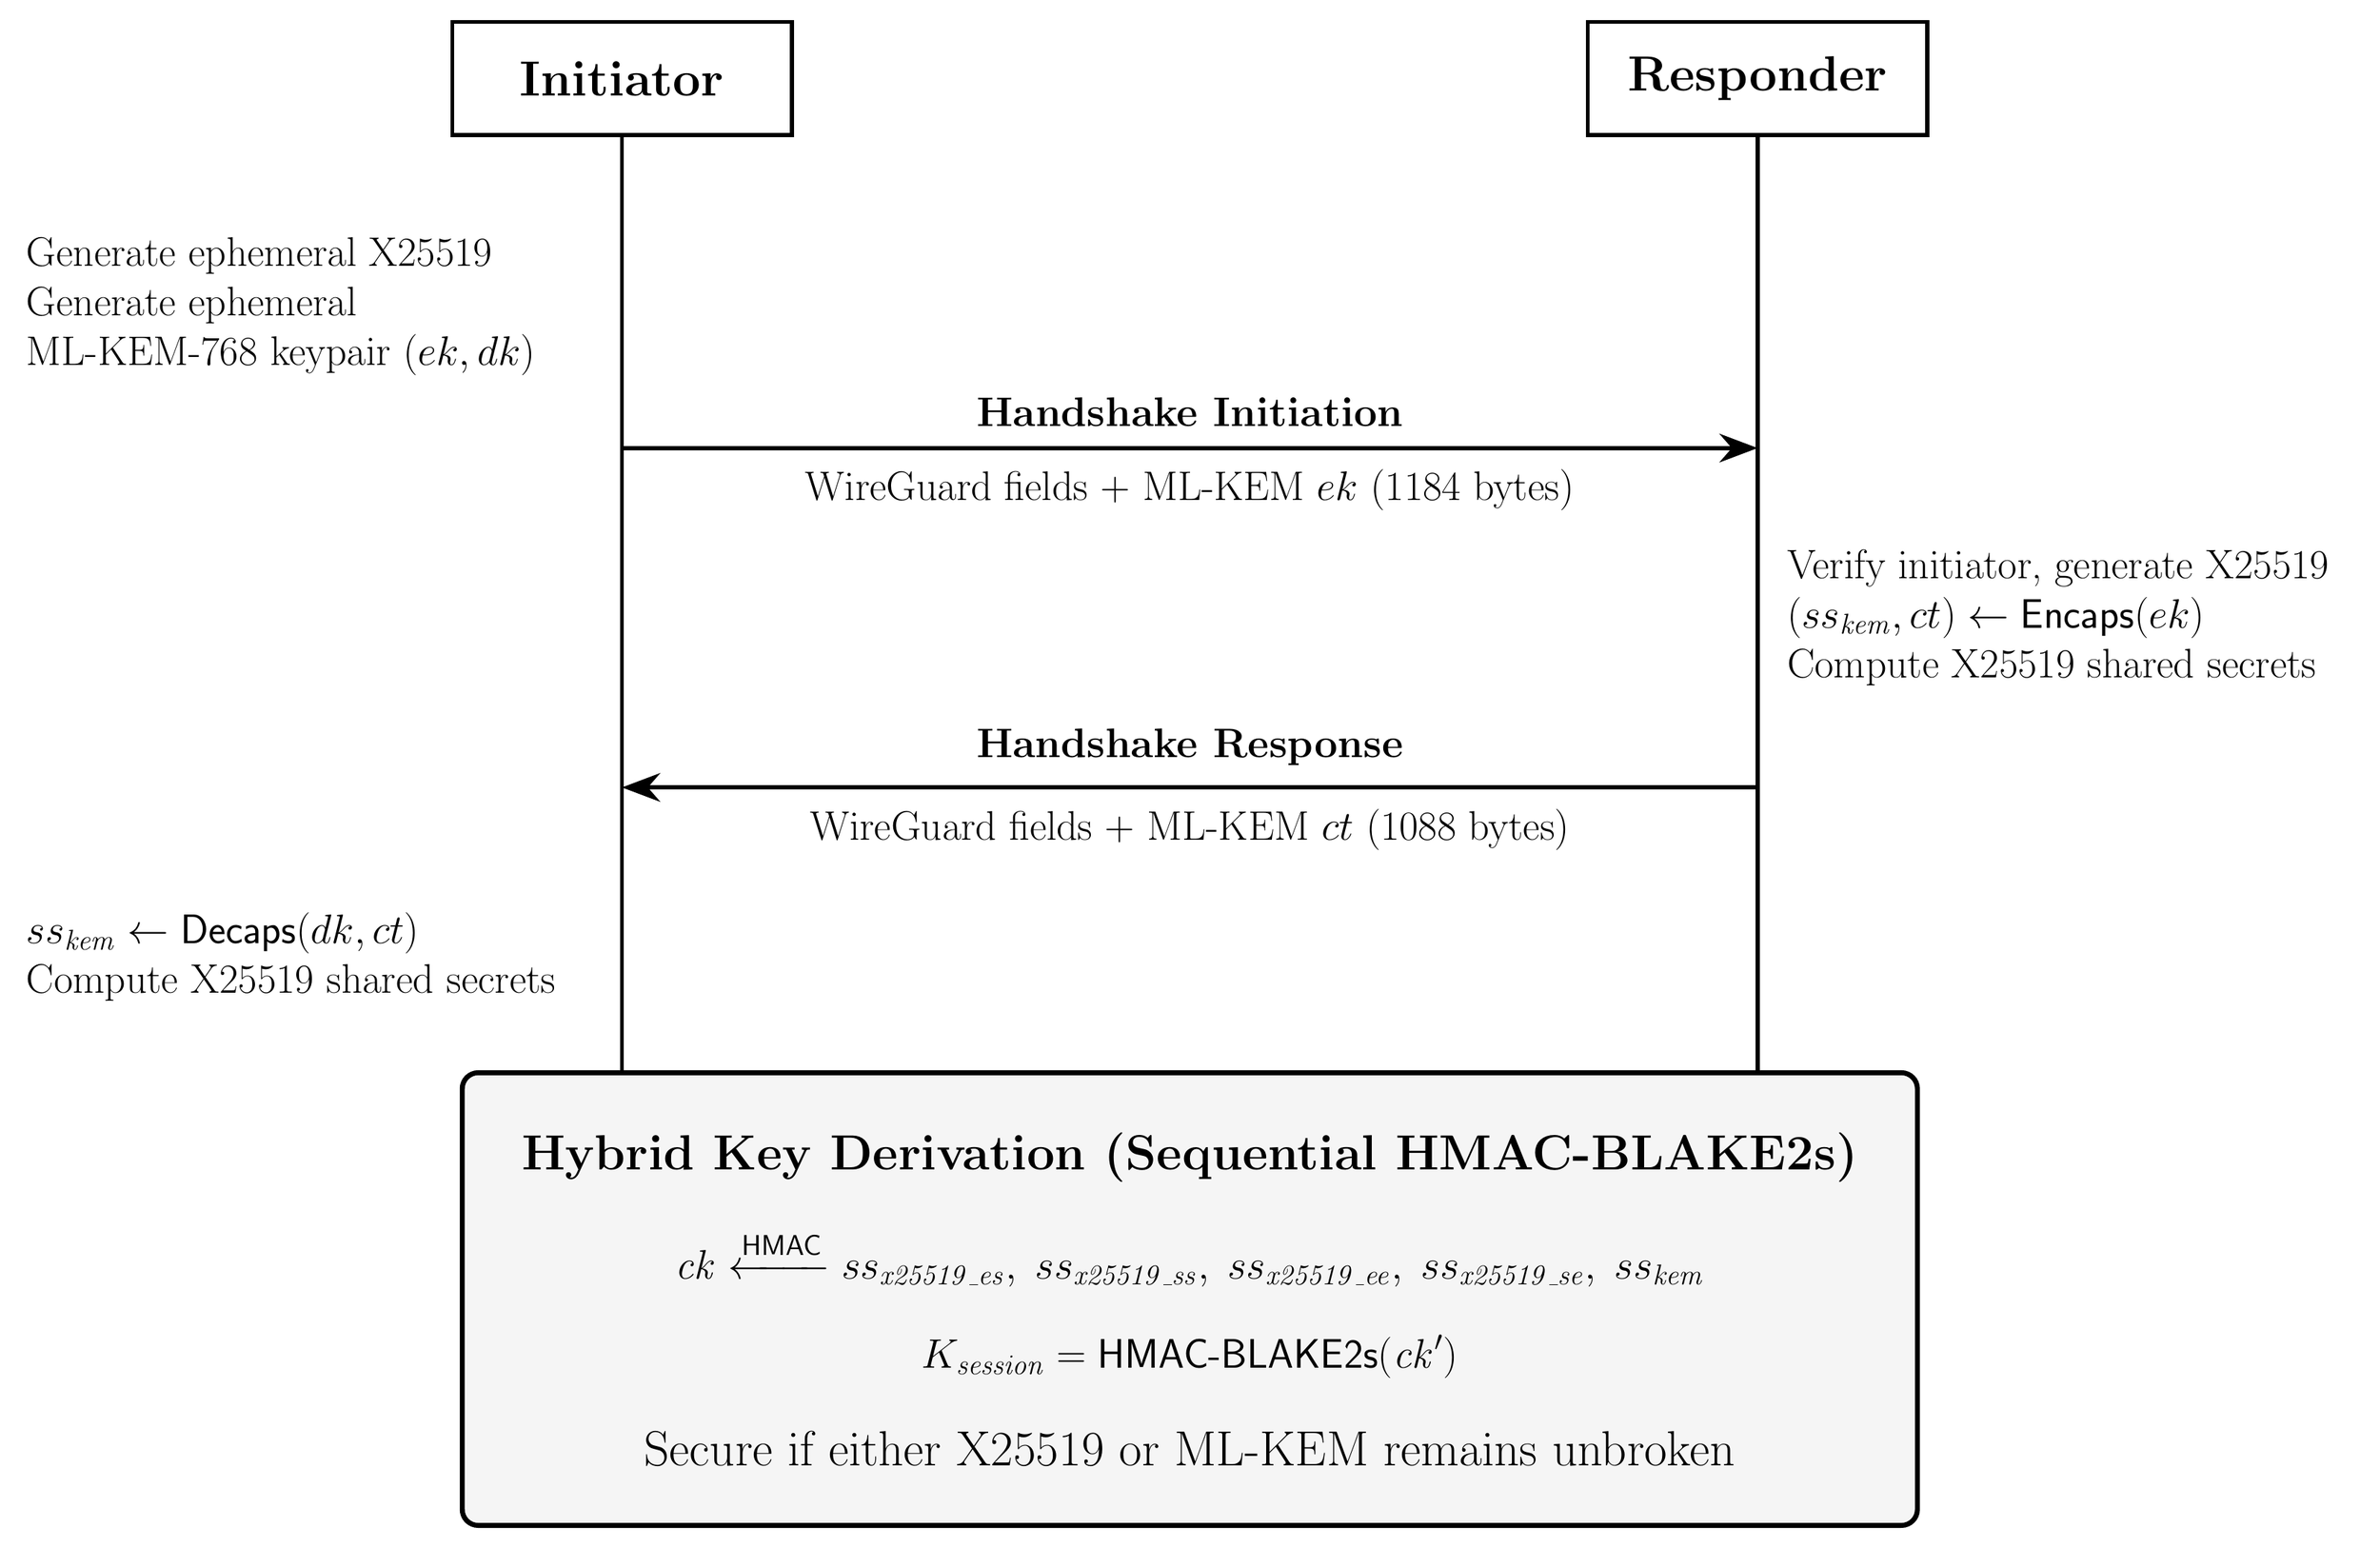
\begin{tikzpicture}[
    box/.style={rectangle, draw=black, line width=2pt, minimum width=6cm, minimum height=2cm, align=center, font=\bfseries\Huge},
    arrow/.style={-{Stealth[scale=1.6]}, line width=2pt},
    msg_label/.style={font=\huge\bfseries, fill=white, inner sep=5pt},
    msg_detail/.style={font=\huge, fill=white, inner sep=5pt},
    action/.style={font=\huge, text width=10cm, align=left},
    timeline/.style={line width=2pt}
]
    % Spacing constants
    \def\colsep{14cm}

    % Nodes
    \node[box] (init) {Initiator};
    \node[box, right=\colsep of init] (resp) {Responder};

    % Timelines
    \draw[timeline] (init.south) -- +(0,-18cm);
    \draw[timeline] (resp.south) -- +(0,-18cm);

    % Row 1: Initiator generates both keypairs
    \coordinate (r1) at ($(init.south)-(0,3cm)$);
    \node[action, anchor=east] at ($(r1)+(-0.4cm,0)$) {Generate ephemeral X25519\\Generate ephemeral\\ML-KEM-768 keypair $(ek, dk)$};

    % Row 2: Message 1 (Initiation with ML-KEM ek)
    \coordinate (m1_start) at ($(init.south)-(0,5.5cm)$);
    \coordinate (m1_end) at ($(resp.south)-(0,5.5cm)$);
    \draw[arrow] (m1_start) -- (m1_end);
    \node[msg_label, above=0.2cm] at ($(m1_start)!0.5!(m1_end)$) {Handshake Initiation};
    \node[msg_detail, below=0.2cm] at ($(m1_start)!0.5!(m1_end)$) {WireGuard fields + ML-KEM $ek$ (1184 bytes)};

    % Row 3: Responder processes and encapsulates
    \coordinate (r3) at ($(resp.south)-(0,8.5cm)$);
    \node[action, anchor=west] at ($(r3)+(0.4cm,0)$) {Verify initiator, generate X25519\\$(ss_{\mathit{kem}}, ct) \gets \textsf{Encaps}(ek)$\\Compute X25519 shared secrets};

    % Row 4: Message 2 (Response with ML-KEM ct)
    \coordinate (m2_start) at ($(resp.south)-(0,11.5cm)$);
    \coordinate (m2_end) at ($(init.south)-(0,11.5cm)$);
    \draw[arrow] (m2_start) -- (m2_end);
    \node[msg_label, above=0.2cm] at ($(m2_start)!0.5!(m2_end)$) {Handshake Response};
    \node[msg_detail, below=0.2cm] at ($(m2_start)!0.5!(m2_end)$) {WireGuard fields + ML-KEM $ct$ (1088 bytes)};

    % Row 5: Initiator decapsulates and computes
    \coordinate (r5) at ($(init.south)-(0,14.5cm)$);
    \node[action, anchor=east] at ($(r5)+(-0.4cm,0)$) {$ss_{\mathit{kem}} \gets \textsf{Decaps}(dk, ct)$\\Compute X25519 shared secrets};

    % Row 6: Hybrid Key Derivation
    \node[draw, line width=2.5pt, fill=gray!8, rounded corners=8pt, below=16.5cm of $(init.south)!0.5!(resp.south)$, anchor=north, align=center, inner sep=30pt, font=\huge] (kdf) {
        \textbf{\Huge Hybrid Key Derivation (Sequential HMAC-BLAKE2s)}\\[24pt]
        $\mathit{ck} \xleftarrow{\textsf{HMAC}} ss_{\mathit{x25519\_es}},\; ss_{\mathit{x25519\_ss}},\; ss_{\mathit{x25519\_ee}},\; ss_{\mathit{x25519\_se}},\; ss_{\mathit{kem}}$\\[20pt]
        $K_{\mathit{session}} = \textsf{HMAC-BLAKE2s}(\mathit{ck}')$\\[24pt]
        {\Huge Secure if either X25519 or ML-KEM remains unbroken}
    };

\end{tikzpicture}
\end{document}
